\section{Benchmarking}

\begin{table*}
    \centering
    \setlength{\tabcolsep}{2pt}
    \renewcommand{\arraystretch}{1.0}
    \caption{\textbf{Geo-time Aware Image Retrieval on images from unseen locations}. Given a query image ($I$) and target time ($t$), the goal is to retrieve an image captured at the \textit{same geographic location} as the query but at the \textit{specified target time}. Our model significantly outperforms prior approaches, demonstrating strong geo-temporal alignment and robustness to temporal variation.  *indicates methods we replicate, closely adhering to protocols outlined by prior work
    }
    \label{tab:sota}
    \begin{tabular}{lccccccc} 
        \toprule
        \multirow{2}{*}{\textbf{Method}} & \multirow{2}{*}{\textbf{Retrieval}} & \multicolumn{3}{c}{\textbf{TIGeR-test-86k}} & \multicolumn{3}{c}{\textbf{CVT}} \\
        \cmidrule(lr){3-5} \cmidrule(lr){6-8}  
        &  &\textbf{R@1 (\%)} & \textbf{R@5 (\%)} & \textbf{R@10 (\%)} & \textbf{R@1 (\%)} & \textbf{R@5 (\%)} & \textbf{R@10 (\%)} \\
        \midrule
        Zhai et al.~\cite{zhai2019learning}* & $It \rightarrow I$ & 1.97 & 7.05 & 11.23 & 0.45 & 1.59 & 2.38 \\
        Zhai et al. w/ CLIP~\cite{zhai2019learning}* & $It \rightarrow I$ & 2.60 & 8.80 & 13.70 & 2.95 & 8.76 & 13.31 \\
        Time-Loc~\cite{Shatwell_2025_ICCV}* & $It \rightarrow I$ & 0.38 & 1.73 & 3.19 & 15.23 & 19.28 & 21.18 \\
        GT-Loc~\cite{Shatwell_2025_ICCV}* & $It \rightarrow I$ & 0.34 & 1.56 & 2.94 & \textbf{16.45} & 20.44 & 22.59 \\
        \midrule
        \textbf{TIGeR (Ours)} & $It \rightarrow I$ & \textbf{3.51} & \textbf{23.30} & \textbf{37.51} & 14.55 & \textbf{24.46} & \textbf{29.98} \\
        \bottomrule
    \end{tabular}
    \vspace{-1em}
\end{table*}

We evaluate \tiger on three retrieval tasks to demonstrate its ability to learn strong and generalizable geo-temporal representations: geo-time aware image retrieval, time-of-capture prediction and geo-localization.

\subsection{Geo-time Aware Image Retrieval}

This task aims to retrieve, from a global gallery, the image that best matches a query in terms of both location and time. Prior work~\cite{Shatwell_2025_ICCV} studied an oracle variant where the ground-truth GPS location $l^Q$ is given, and the query is formed by fusing the location and target time $t^Q$ embeddings. Here we consider a more challenging and realistic setting: given a query image $I^Q$ and target time $t^Q$, the goal is to retrieve an image $\{I_i^G\}_{i=1}^N$ captured at the same physical location as $I^Q$ and at time $t^Q$. In this case, the model must infer and preserve location identity directly from the image, rather than relying on explicit GPS.

We address this problem by encoding the image and time with \tiger and fusing their embeddings into a unified geo-temporal representation. We precompute gallery embeddings $\bar{\mathbf{v}}_i^G = f(I_i^G)$ and, at inference, obtain the fused query representation $\bar{\mathbf{vt}}^Q = f(I^Q, t^Q)$. Retrieval is then performed by maximizing cosine similarity:
\begin{equation}
    (I^Q)^* = \argmax_{I^G} \big( f(I^Q, t^Q)^\top f(I^G) \big).
    \label{eq:optim-gtret}
\end{equation}

We evaluate on two complementary benchmarks: our \textsc{TIGeR-test-86k} split and a balanced partition of CVT~\cite{salem2020dynamic} across hemispheres. \textsc{TIGeR-test-86k} is built from webcams with multiple observations of the same camera across the year, enabling fine-grained geo-temporal retrieval at fixed locations but varying times. CVT instead consists of social media images at arbitrary locations and times, without repeated cameras; here, retrieval is considered correct if the result lies within $125$\,km of the query location and matches the specified time.

We compare \tiger against two main baselines. The first is the triple-encoder classifier of Zhai et al.~\cite{zhai2019learning}, originally proposed for joint geo-location and time-of-capture classification. In addition to the original InceptionV2~\cite{szegedy2016rethinking} backbone, we also evaluate a stronger variant with a CLIP ViT-L/14~\cite{clip} backbone for fair comparison. Following~\cite{Shatwell_2025_ICCV}, we adapt this model to retrieval by first predicting the query geo-location class $\hat{l}^Q$, then computing location and time posteriors $P(l \mid I_i^G)$ and $P(t \mid I_i^G)$ for each gallery image and defining
\[
\mathrm{score}(I_i^G) = P(l = \hat{l}^Q \mid I_i^G)\, P(t = t^Q \mid I_i^G),
\]
which is used to rank the gallery.

The second baseline is GT-Loc~\cite{Shatwell_2025_ICCV}, which maps locations, images, and times into a shared feature space but lacks \tiger's multimodal transformer. Here we encode image and time independently and perform late fusion by averaging their embeddings, which cannot explicitly model higher-order interactions between geo-location and time.

Table~\ref{tab:sota} reports quantitative results. \tiger consistently outperforms all baselines, achieving higher recall at most ranks on both datasets. This indicates that the learned representations are well aligned across visual, temporal, and geo-location modalities, and that the fused embeddings successfully encode both location and time information rather than over-emphasizing purely semantic visual similarity. Qualitative examples comparing \tiger and the baselines are shown in Figure~\ref{fig:qualitative}. We show additional examples on the supplementary section~\ref{sup:qualitative}.


\subsection{Time Prediction and Geo-localization}

In this task, the objective is to estimate both the geo-location and time-of-capture of a query image by comparing its embedding against dedicated galleries of location and time embeddings, respectively, and selecting the most compatible entries according to cosine similarity.

Let $I^{Q}$ be a query image and let $\{x_i^{G}\}_{i=1}^{N_G}$ denote a gallery of targets from a modality $x$ (either GPS coordinates or timestamps). Our model produces an image embedding $\bar{\mathbf{v}}^{Q}\!\in\!\mathbb{R}^{d}$ and a gallery embedding $\mathbf{x}^{G}_i\!\in\!\mathbb{R}^{d}$ for each gallery item. In addition, a modality-specific classifier predicts a probability vector $\hat{\mathbf{y}}$ over $B$ coarse classes (e.g., HEALPix bins for GPS or time bins for timestamps). We write $b(x_i^{G})\!\in\!\{1,\dots,B\}$ for the class index associated with gallery item $x_i^{G}$.

We combine a continuous retrieval signal with a discrete prior. Treat the cosine similarity as a temperature-scaled log-likelihood of a match, and the classifier output as a prior over classes. The resulting posterior-like score for each gallery item $x_i^{G}$ is
\begin{equation}
    \label{eq:poe-score}
    \mathrm{score}(x_i^{G})
    \;=\;
    \frac{(\bar{\mathbf{v}}^{Q})^{\top}\mathbf{x}^{G}_i}{\psi}
    \;+\;
    \beta(I^{Q})\,\log P\!\left(b(x_i^{G}) \mid I^{Q}\right),
\end{equation}
where $\psi\!>\!0$ is a temperature parameter and $\beta(I^{Q})\!\ge\!0$ controls the influence of the classifier prior for the query.

A fixed $\beta$ can help on easy (confident) queries and hurt on hard (uncertain) ones. We therefore make $\beta$ \emph{query-adaptive} using the classifier entropy:
\begin{equation}
    \label{eq:beta-entropy}
    \beta(I^{Q})
    \;=\;
    \beta_{\max}\!\left(
    1 - \frac{H(\hat{\mathbf{y}})}{\log B}
    \right),
\end{equation}
where $H(\hat{\mathbf{y}})$ is the Shannon entropy and $\log B$ the maximum entropy for $B$ classes. Thus, $\beta(I^{Q})\!\in[0,\beta_{\max}]$: it approaches $\beta_{\max}$ when the classifier is confident (low entropy) and decreases toward $0$ when it is uncertain (high entropy).

Equation~\eqref{eq:poe-score} allows the retrieval term to \emph{pull} fine-grained neighbors while the prior \emph{guides} the search toward plausible classes. The entropy-adaptive weighting in \eqref{eq:beta-entropy} ensures the prior has strong influence only when it is informative, mitigating boundary effects and domain shift.

In the time prediction task, rather than conditioning onlt on the image embedding $\bar{\mathbf{v}}^{Q}$, we can optionally incorporate the known location as auxiliary input. In this setting, we use the fused embedding $\bar{\mathbf{vl}}^{Q}=f(I^{Q},G^{Q})$ as the query representation and compute cosine similarity against gallery time embeddings. This variant often improves temporal prediction accuracy by constraining retrieval to locations consistent with the provided GPS context.

Tables~\ref{tab:time-pred} and~\ref{tab:geolocalization} summarize the performance of our method on time prediction and geo-localization, respectively. Overall, \tiger achieves state-of-the-art results on both tasks. For time-of-capture prediction, \tiger consistently outperforms prior methods on both month and hour estimation. Moreover, when geo-location is provided as an auxiliary input and fused with the image representation, performance improves substantially. This behavior is expected, as the visual appearance of time is strongly coupled with latitude and season (e.g., higher latitudes exhibit more pronounced seasonal variation than regions near the Equator).

For geo-localization, \tiger also attains competitive performance compared to strong baselines. However, in this setting, using time as an auxiliary signal does not always lead to further gains. Unlike location, time-of-capture is a comparatively weak and ambiguous cue for disambiguating places: many geographically distant locations can share similar illumination and seasonal appearance at a given time, and the time predictions themselves may be noisy. Incorporating this uncertain temporal signal can therefore introduce additional variance or bias the model toward spurious correlations, which sometimes offsets the benefits of joint time–location reasoning for geo-localization.

\begin{table}[t]
\centering
\setlength{\aboverulesep}{0pt}
\setlength{\belowrulesep}{0pt}
\caption{\textbf{Time prediction} on unseen cameras. *indicates methods we replicate, closely adhering to protocols outlined by prior work.}
\label{tab:time-pred}
\begingroup
\setlength{\tabcolsep}{1pt}
\resizebox{\linewidth}{!}{
\begin{tabular}{lccccc} 
\toprule
\multirow{3}{*}{\textbf{Method}} & \multirow{3}{*}{\textbf{Retrieval}}
  & \multicolumn{2}{c}{\textbf{TIGeR-test-86k}}
  & \multicolumn{2}{c}{\textbf{CVT-test}} \\
\cmidrule(lr){3-4} \cmidrule(lr){5-6}
                & 
  & \textbf{ToY} & \textbf{ToD} 
  & \textbf{ToY} & \textbf{ToD}  \\
                & 
  & \textbf{Error}$\downarrow$ & \textbf{Error}$\downarrow$
  & \textbf{Error}$\downarrow$ & \textbf{Error}$\downarrow$  \\
\midrule

Zhai et al.~\cite{zhai2019learning}*                & $I \rightarrow t$ & 68.38 & 3.97 & 87.37 & 3.28  \\
Zhai et al. w/ CLIP ~\cite{zhai2019learning}*        & $I \rightarrow t$ & 57.51 & 3.22 & 68.95 & 2.8  \\
Time-Loc~\cite{Shatwell_2025_ICCV}*   & $I \rightarrow t$ & 74.87 & 4.02 & 65.10 & 2.86 \\
GT-Loc~\cite{Shatwell_2025_ICCV}*    & $I \rightarrow t$  & 74.58 & 3.52 & 78.95 & \textbf{2.68} \\

\midrule

\textbf{TIGeR (Ours)}    & $I \rightarrow t$  & \textbf{51.49} & \textbf{3.13} & \textbf{62.88} & 2.73 \\

\midrule
Zhai et al.~\cite{zhai2019learning}*               & $Il \rightarrow t$ & 66.36 & 3.88 & 73.15 & 3.15  \\
Salem et al.~\cite{salem2022timestamp}*               & $Il \rightarrow t$ & 74.29 & 3.57 & 75.48 & 3.1  \\
% \midrule
Zhai et al. w/ CLIP~\cite{zhai2019learning}*        & $Il \rightarrow t$ & 55.15 & 3.19 & 60.42 & 2.77  \\
Salem et al. w/ CLIP~\cite{salem2022timestamp}*       & $Il \rightarrow t$ & 55.4 & 3.24 & 64.05 & 2.71  \\

\midrule

\textbf{TIGeR (Ours)}    & $Il \rightarrow t$ & \textbf{48.86} & \textbf{3.06} & \textbf{47.00} & \textbf{2.35} \\

\bottomrule
\end{tabular}}
\endgroup
\end{table}

\begin{table}
    \centering
    \caption{\textbf{Geo-localization accuracy}. *indicates methods we replicate, closely adhering to protocols outlined by prior work.}
    \label{tab:geolocalization}
    \resizebox{\columnwidth}{!}{%
    \begin{tabular}{lccccc}
        \toprule
        \multirow{2}{*}{\textbf{Method}} &
        \multirow{2}{*}{\textbf{Retrieval}} &
        \multicolumn{2}{c}{\textbf{TIGeR-test-86k}} &
        \multicolumn{2}{c}{\textbf{CVT-test}} \\
        \cmidrule(lr){3-4}\cmidrule(lr){5-6}
        & & \textbf{200 km} & \textbf{750 km} &
            \textbf{200 km} & \textbf{750 km} \\
        \midrule
        Zhai et al.~\cite{zhai2019learning}*          & $I \rightarrow l$  & 22.05 & 46.20 &  3.50 & 10.50 \\
        Zhai et al. w/ CLIP~\cite{zhai2019learning}*   & $I \rightarrow l$  & 28.58 & 64.85 & 23.13 & 57.74 \\
        GeoCLIP~\cite{vivanco2024geoclip}              & $I \rightarrow l$  & 21.58 & 37.58 & 43.62 & 60.77 \\
        GT-Loc~\cite{Shatwell_2025_ICCV}*               & $I \rightarrow l$  & 21.07 & 35.93 & 42.63 & 59.49 \\
        \midrule
        \textbf{TIGeR (Ours)}        & $I \rightarrow l$  & \textbf{48.63} & \textbf{65.61} & \textbf{51.90} & \textbf{66.53} \\
        \midrule
        Zhai et al.~\cite{zhai2019learning}*          & $It \rightarrow l$ & 21.99 & 46.62 &  4.46 & 13.41 \\
        Zhai et al. w/ CLIP~\cite{zhai2019learning}*   & $It \rightarrow l$ & 28.83 & 65.16 & 23.82 & 58.97 \\
        \midrule
        \textbf{TIGeR (Ours)}        & $It \rightarrow l$ & \textbf{48.34} & \textbf{64.51} & \textbf{53.40} & \textbf{67.15} \\
        \bottomrule
    \end{tabular}%
    }
\end{table}


\begin{figure}[t]
\begin{center}
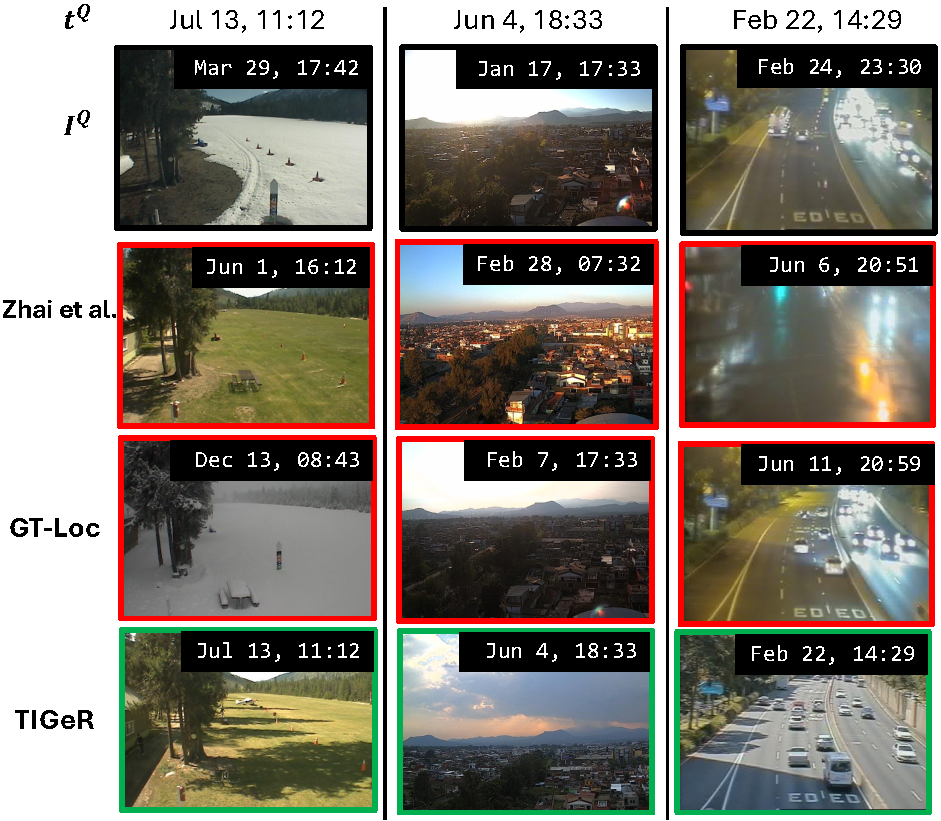
\includegraphics[width=\linewidth]{figures/tiger_qual_crop.pdf}
\end{center}
\caption{\textbf{Qualitative results on geo-time aware image retrieval with images from unseen locations}. Given a query image $I^Q$ and a target time $t^Q$ (shown above each column), the goal is to retrieve an image captured at the \textit{same location} as the query but at the specified target time. For visualization, the actual time-of-capture for each image is overlaid on top of it. 
Each row shows top-1 retrieval results from different methods. While prior approaches (Zhai et al.~\cite{zhai2019learning}, GT-Loc~\cite{Shatwell_2025_ICCV}) often retrieve images captured at incorrect times, our \textsc{\tiger} model accurately retrieves images corresponding to the target time while maintaining location consistency. Best viewed in color. 
}
\label{fig:qualitative}
\end{figure}


\begin{table}[h]
    \centering
    \caption{Cumulative ablation study on the components of \tiger.}
    \label{tab:ablations-components}
    \resizebox{\columnwidth}{!}{%
    \begin{tabular}{lccc} 
        \toprule
        
        \multirow{2}{*}{\textbf{Setting}} &
        \multicolumn{1}{c}{\textbf{Month}} &
        \multicolumn{1}{c}{\textbf{Hour}} &
        \multicolumn{1}{c}{\textbf{Geo-location}} \\
        & \multicolumn{1}{c}{\textbf{Error}} &
          \multicolumn{1}{c}{\textbf{Error}} &
          \multicolumn{1}{c}{\textbf{Error (km)}} \\
        \midrule
        Base model                      & 76.77 & 3.10 & 668.97 \\
        + multi-modal transformer       & 57.58 & 2.98 & 238.58 \\
        + Classification heads          & 57.20 & 2.95 & 234.53 \\
        + Entropy adaptive reranking    & 57.20 & 2.93 & 203.93 \\
        \bottomrule
    \end{tabular}%
    }
\end{table}

\subsection{Ablation Analysis}

We conduct an ablation study to quantify the contribution of each component of \tiger on geo-localization and time-of-capture prediction. For both tasks, we report errors averaged over \textsc{TIGeR-test-86k} and CVT-test. For geo-localization, we use mean geodetic error (in kilometers) rather than recall at distance thresholds, as this yields a single, directly comparable metric.

Table~\ref{tab:ablations-components} summarizes the results. We start from a \emph{base model} that includes image, location, and time encoders trained with only two contrastive losses, analogous to GT-Loc~\cite{Shatwell_2025_ICCV}. Adding the \emph{multi-modal transformer} together with the five cross-modal contrastive losses from Eq.~\ref{eq:contrastive-losses} yields the largest performance gain across both temporal and geo-location errors, highlighting the importance of joint geo-temporal modeling. Next, we introduce \emph{classification heads} as auxiliary supervision during training, which provides a modest additional improvement. Finally, we leverage these heads at test time through our \emph{entropy-adaptive reranking} scheme, which uses the classifier predictions as a confidence-weighted prior. This step produces a substantial reduction in geo-localization error, resulting in the full \tiger model. Additional ablations and analyses are provided in the supplementary section~\ref{sup:ablations}.

